\documentclass[10pt]{beamer}
\usepackage{iftex}
\ifPDFTeX
\usepackage[T2A]{fontenc}
\usepackage[utf8]{inputenc} % Кодировка utf-8, cp1251 и т.д.
\usepackage[english,russian]{babel}
\else
  \RequirePackage{polyglossia}
 \RequirePackage{luatextra}
  \defaultfontfeatures{Ligatures=TeX,Numbers=Lining,Scale=MatchLowercase}

  \setmainfont{Times New Roman}
  \setsansfont{Calibri}
  \setmonofont{Fira Code}

  %\setmathfont{Cambria Math}%

  \newfontfamily{\cyrillicfont}{Times New Roman}
  \newfontfamily{\cyrillicfontrm}{Times New Roman}
  \newfontfamily{\cyrillicfonttt}{Fira Code}
  \newfontfamily{\cyrillicfontsf}{Fira Sans Regular}
\fi

\usepackage{amsmath,amssymb,longtable,hhline}
\usepackage{mathrsfs}
\usepackage{xcolor}
\usepackage{listings}
\usepackage{hyperref}
\usepackage{multicol}
\usepackage{anyfontsize}
\usepackage{minted}
%\usepackage{enumitem}

% \setlist[description]{leftmargin=0pt,labelindent=\parindent}

\usemintedstyle{tango}
\newcommand{\ltprgsize}{\fontsize{5}{5}\selectfont}
\setminted{fontsize=\ltprgsize,mathescape}

\definecolor{mygreen}{rgb}{0,0.6,0}
\definecolor{mygray}{rgb}{0.5,0.5,0.5}
\definecolor{mymauve}{rgb}{0.58,0,0.82}

\hypersetup{
    bookmarks=true,         % show bookmarks bar?
    unicode=true,           % non-Latin characters in Acrobat’s bookmarks
    pdftoolbar=false,        % show Acrobat’s toolbar?
    pdfmenubar=false,        % show Acrobat’s menu?
    pdffitwindow=false,     % window fit to page when opened
    pdfstartview={FitH},    % fits the width of the page to the window
    pdftitle={Компьютерная алгебра в задачах оптимизации},    % title
    pdfauthor={Evgeny Cherkashin, Seseg Badmatsyrenova},     % author
    pdfsubject={symbolic computations},   % subject of the document
    pdfnewwindow=true,      % links in new PDF window
    colorlinks=true,       % false: boxed links; true: colored links
    linkcolor=red,          % color of internal links (change box color with linkbordercolor)
    citecolor=green,        % color of links to bibliography
    filecolor=magenta,      % color of file links
    urlcolor=blue           % color of external links
}

\lstset{language=Python,
  basicstyle=\footnotesize\ttfamily,        % the size of the fonts that are used for the code
  breakatwhitespace=false,         % sets if automatic breaks should only happen at whitespace
  breaklines=true,                 % sets automatic line breaking
  captionpos=b,                    % sets the caption-position to bottom
  commentstyle=\color{mygreen},    % comment style
  escapeinside={\%*}{*)},          % if you want to add LaTeX within your code
  extendedchars=true,              % lets you use non-ASCII characters; for 8-bits encodings only, does not work with UTF-8
%  frame=single,                    % adds a frame around the code
  keepspaces=true,                 % keeps spaces in text, useful for keeping indentation of code (possibly needs columns=flexible)
  keywordstyle=\color{blue},       % keyword style
%  numbers=left,                    % where to put the line-numbers; possible values are (none, left, right)
  numbersep=5pt,                   % how far the line-numbers are from the code
  numberstyle=\tiny\color{mygray}, % the style that is used for the line-numbers
  rulecolor=\color{black},         % if not set, the frame-color may be changed on line-breaks within not-black text (e.g. comments (green here))
  showspaces=false,                % show spaces everywhere adding particular underscores; it overrides 'showstringspaces'
  showstringspaces=false,          % underline spaces within strings only
  showtabs=false,                  % show tabs within strings adding particular underscores
  stepnumber=2,                    % the step between two line-numbers. If it's 1, each line will be numbered
  stringstyle=\color{mymauve},     % string literal style
  tabsize=2,                       % sets default tabsize to 2 spaces
%  title=\lstname                   % show the filename of files included with \lstinputlisting; also try caption instead of
}
\usepackage{pifont}

\usetheme{Warsaw}
\usecolortheme{crane}
%\useinnertheme{rectangles}
\setbeamertemplate{itemize item}{\scriptsize\hbox{\donotcoloroutermaths\ding{113}}}
\setbeamertemplate{itemize subitem}{\tiny\raise1.5pt\hbox{\donotcoloroutermaths$\blacktriangleright$}}
\setbeamertemplate{itemize subsubitem}{\tiny\raise1.5pt\hbox{\donotcoloroutermaths$\blacktriangleright$}}
\setbeamertemplate{enumerate item}{\insertenumlabel.}
\setbeamertemplate{enumerate subitem}{\insertenumlabel.\insertsubenumlabel}
\setbeamertemplate{enumerate subsubitem}{\insertenumlabel.\insertsubenumlabel.\insertsubsubenumlabel}
\setbeamertemplate{enumerate mini template}{\insertenumlabel}

\beamertemplatenavigationsymbolsempty

\usepackage{iftex,ifxetex}
\ifPDFTeX
  \usepackage[utf8]{inputenc}
  \usepackage[T1]{fontenc}
  \usepackage[russian]{babel}
  \usepackage{lmodern}
  \usefonttheme{serif}
\else
  \ifluatex
    \usepackage{unicode-math}
    \defaultfontfeatures{Ligatures=TeX,Numbers=OldStyle}
    \setmathfont{Latin Modern Math}
    \setsansfont{Linux Biolinum O}
    \setmonofont{Fira Code}
    \usefonttheme{professionalfonts}
    % \setmathfont[
    %     Ligatures=TeX,
    %     Scale=MatchLowercase,
    %     math-style=upright,
    %     vargreek-shape=unicode
    %     ]{euler.otf}
  \fi
\fi

%\useoutertheme{split}
%\useinnertheme{rounded}
\setbeamertemplate{background canvas}[vertical shading][bottom=white!80!cyan!20,top=cyan!10]
%\setbeamertemplate{sidebar canvas left}[horizontal shading][left=white!40!black,right=black]

\graphicspath{{pics/}}


% --------------------------

% Продукт (Конкуренты, свойства)
% Графический аспект
% Технические аспекты
% Содержание сайта
% Дополнительная информация
% Контактная информация


\begin{document}
\title{Интернет--сервис сбора данных для централизованных бухгалтерий}
\author{Е.~А.~Черкашин}
\institute[ИДСТУ СО РАН, ИрНИТУ, ИМЭИ ИГУ]{ИДСТУ им.~В.~М.~Матросова СО РАН, ИрНИТУ, ИМЭИ ИГУ}
\date[2019]{{}\\[1.5cm]
%<<>>\\
26 января 2019, Иркутск
}
%\date{\today}
\maketitle

\begin{frame}
  \frametitle{Сбор данных с подчиненных учреждений}
  \begin{columns}
    \begin{column}{0.6\linewidth}
  \begin{block}{Основные функции системы}
  \begin{itemize}
  \item Подготовка опросных форм сбора данных из документов \textbf{EXCEL}, \ldots,
  \item Проведение опроса подчиненных учреждений в заданные сроки,
  \item Ведение БД ответов, подготовка отчетов (документов).
  \end{itemize}
\end{block}
  \begin{block}{Конкуренты}
  \begin{itemize}
  \item Google forms -- просты, нет необходимых функций;
  \item 1С Бухгалтерия Web -- надо реализовывать индивидуально;
  \item Собственная разработка -- требует наличие программиста.
  \end{itemize}
\end{block}
  \end{column}
  \begin{column}{0.4\linewidth}
  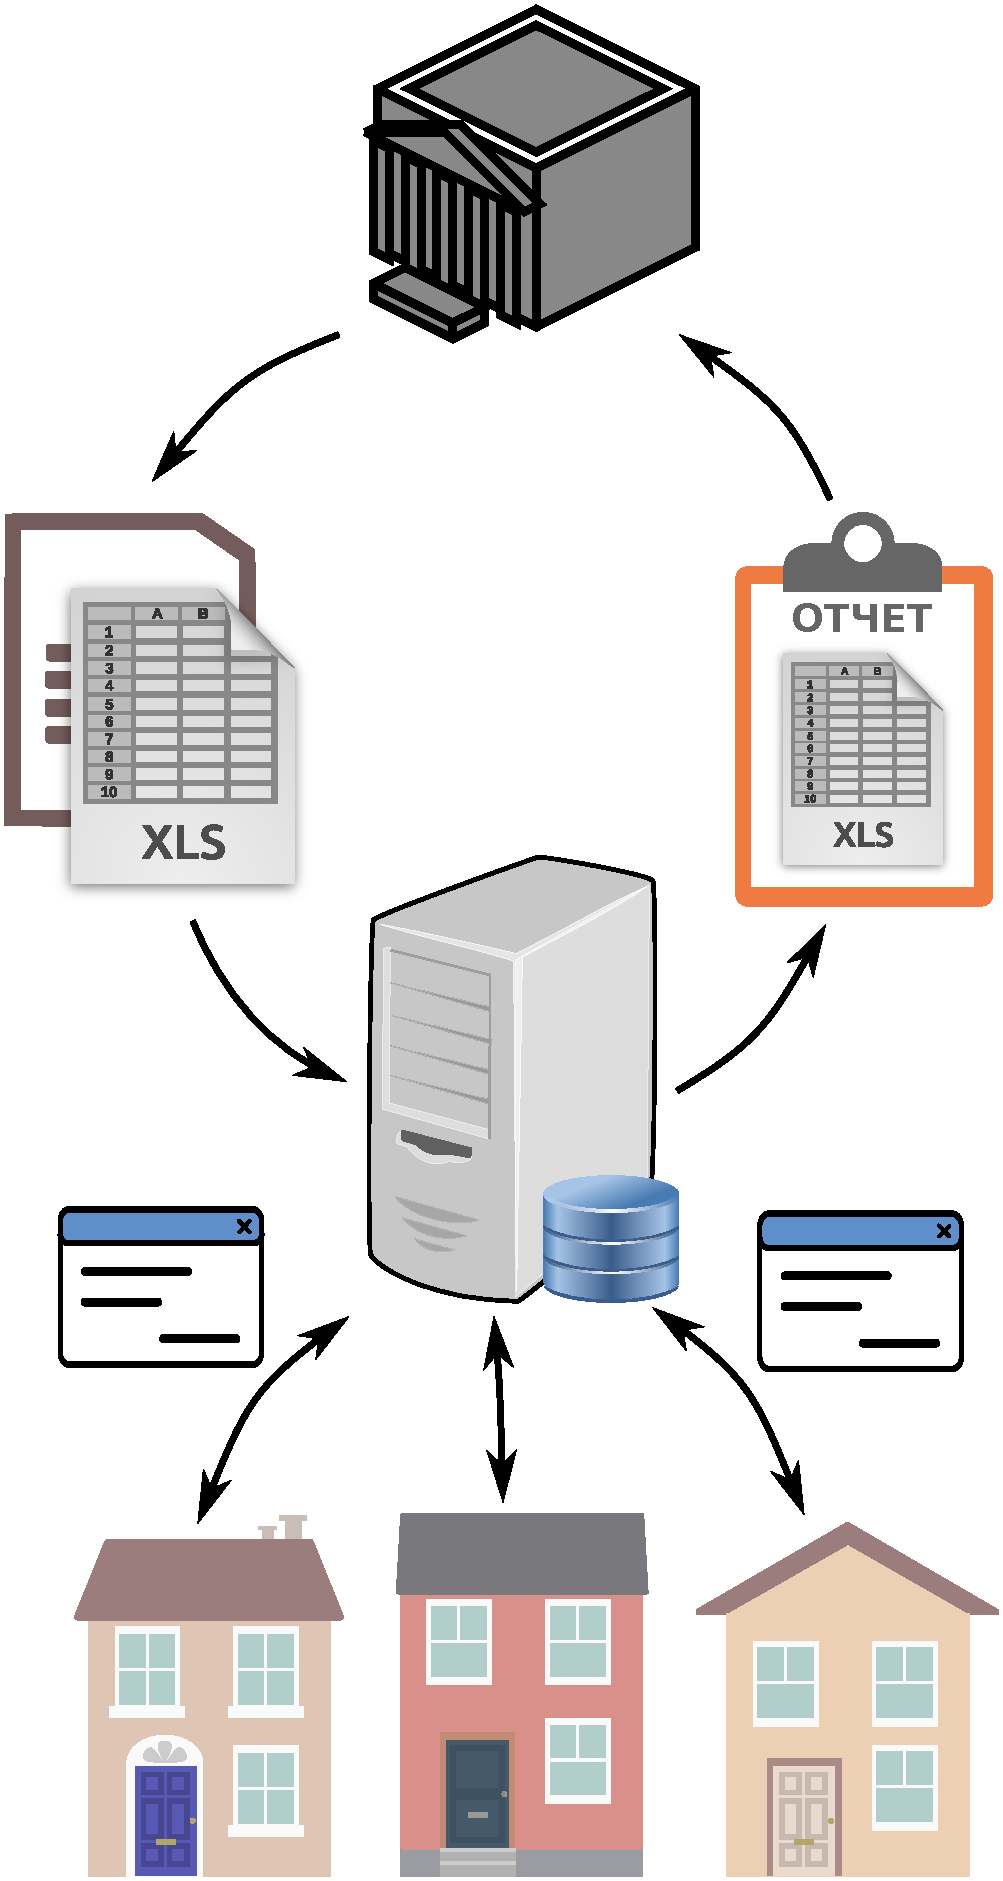
\includegraphics[width=1\linewidth]{pics/mku-task.pdf}
    \end{column}
  \end{columns}
\end{frame}

\begin{frame}
  \frametitle{Пример \textbf{документа} и его формы опроса}
  \centering
  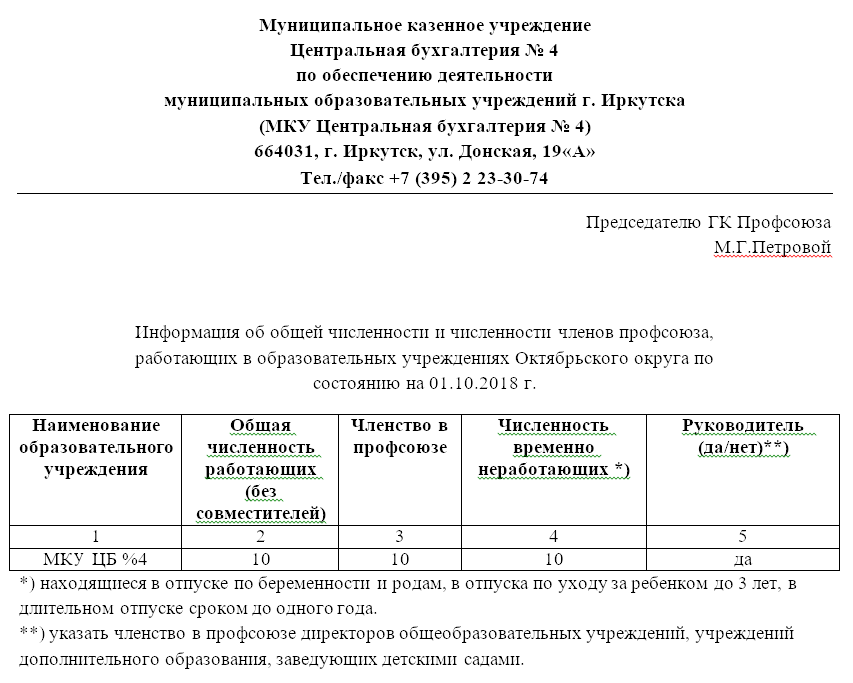
\includegraphics[width=1\linewidth]{pics/quest-source.png}
\end{frame}

\begin{frame}
  \frametitle{Пример документа и его \textbf{формы опроса}}
  \centering
  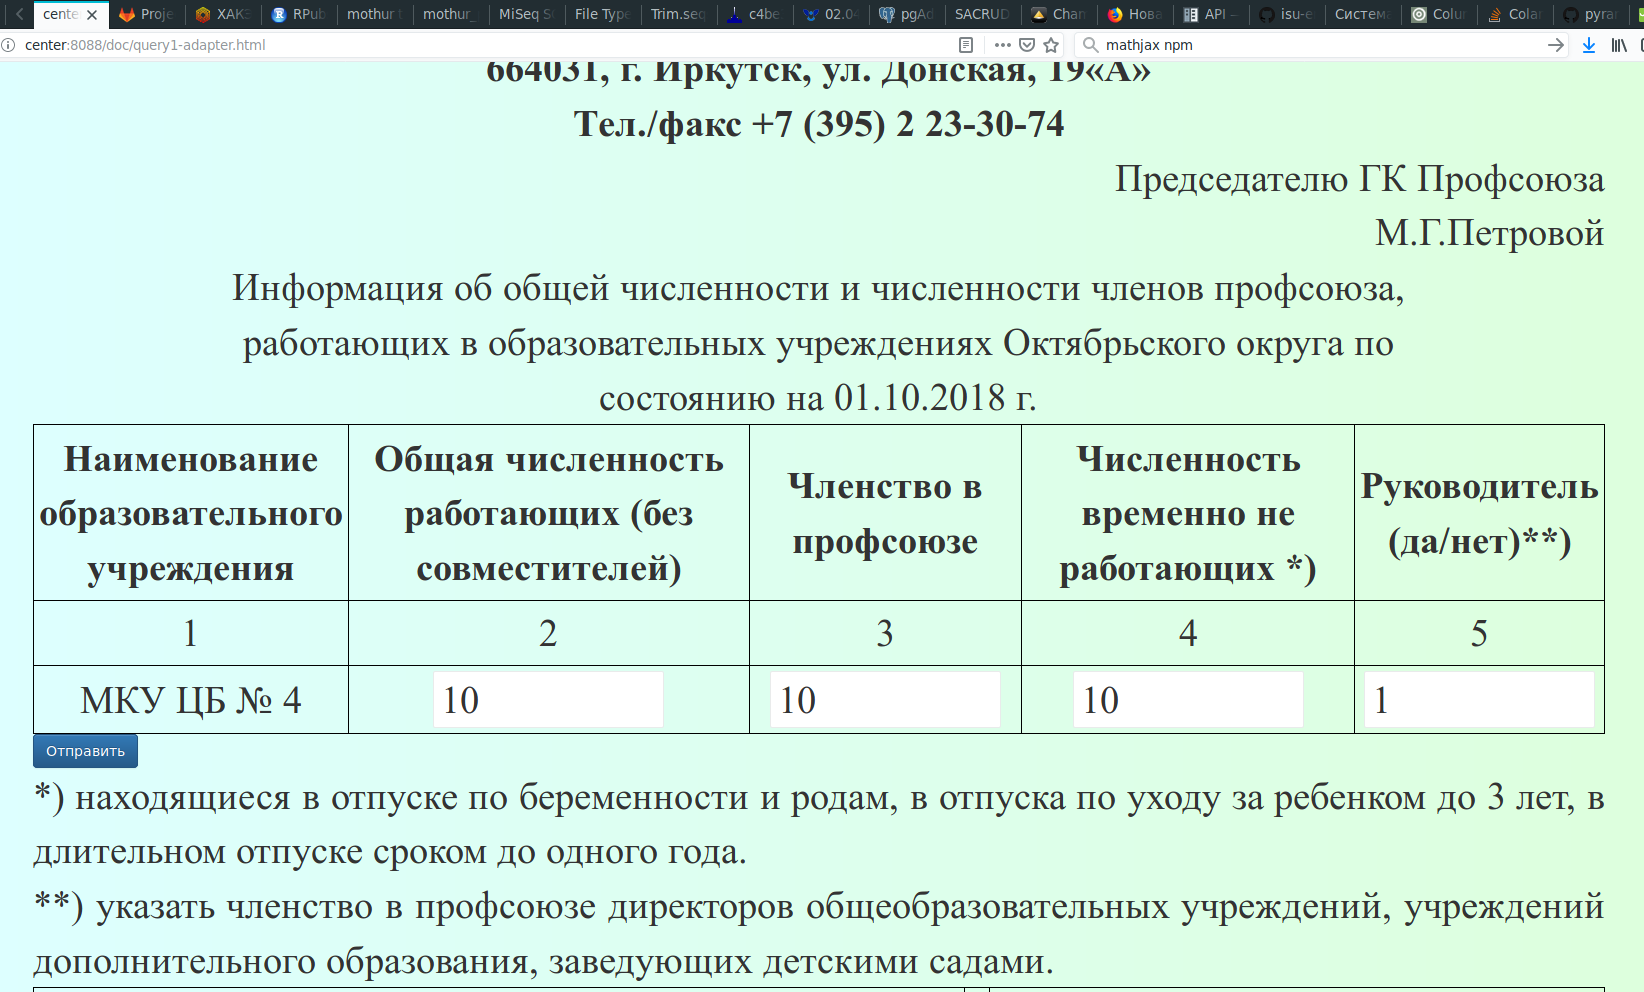
\includegraphics[width=1\linewidth]{pics/quest-form.png}
\end{frame}

\begin{frame}
  \frametitle{Основной интерфейс}
  % \centering
  \hspace{-5em}
  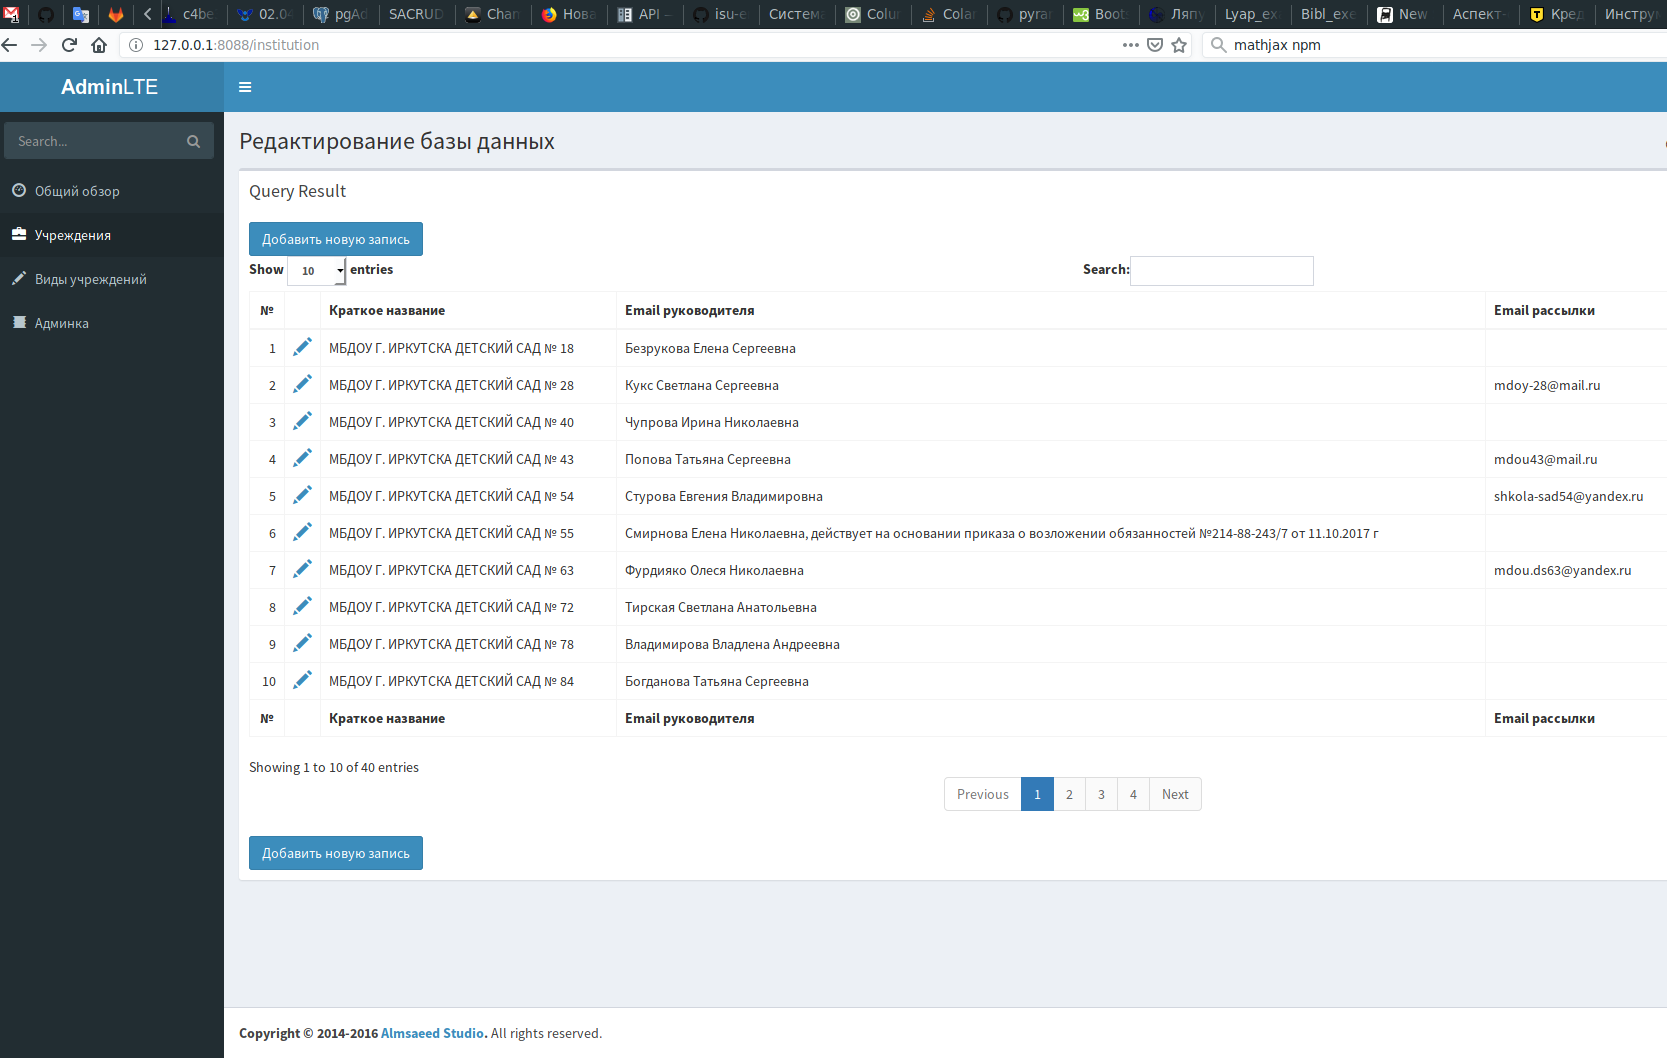
\includegraphics[width=1.3\linewidth]{pics/quest-table-shot.png}
\end{frame}

\begin{frame}
  \frametitle{Инфраструктура интеграции сервисов анализа и принятия решения}
  \centering
  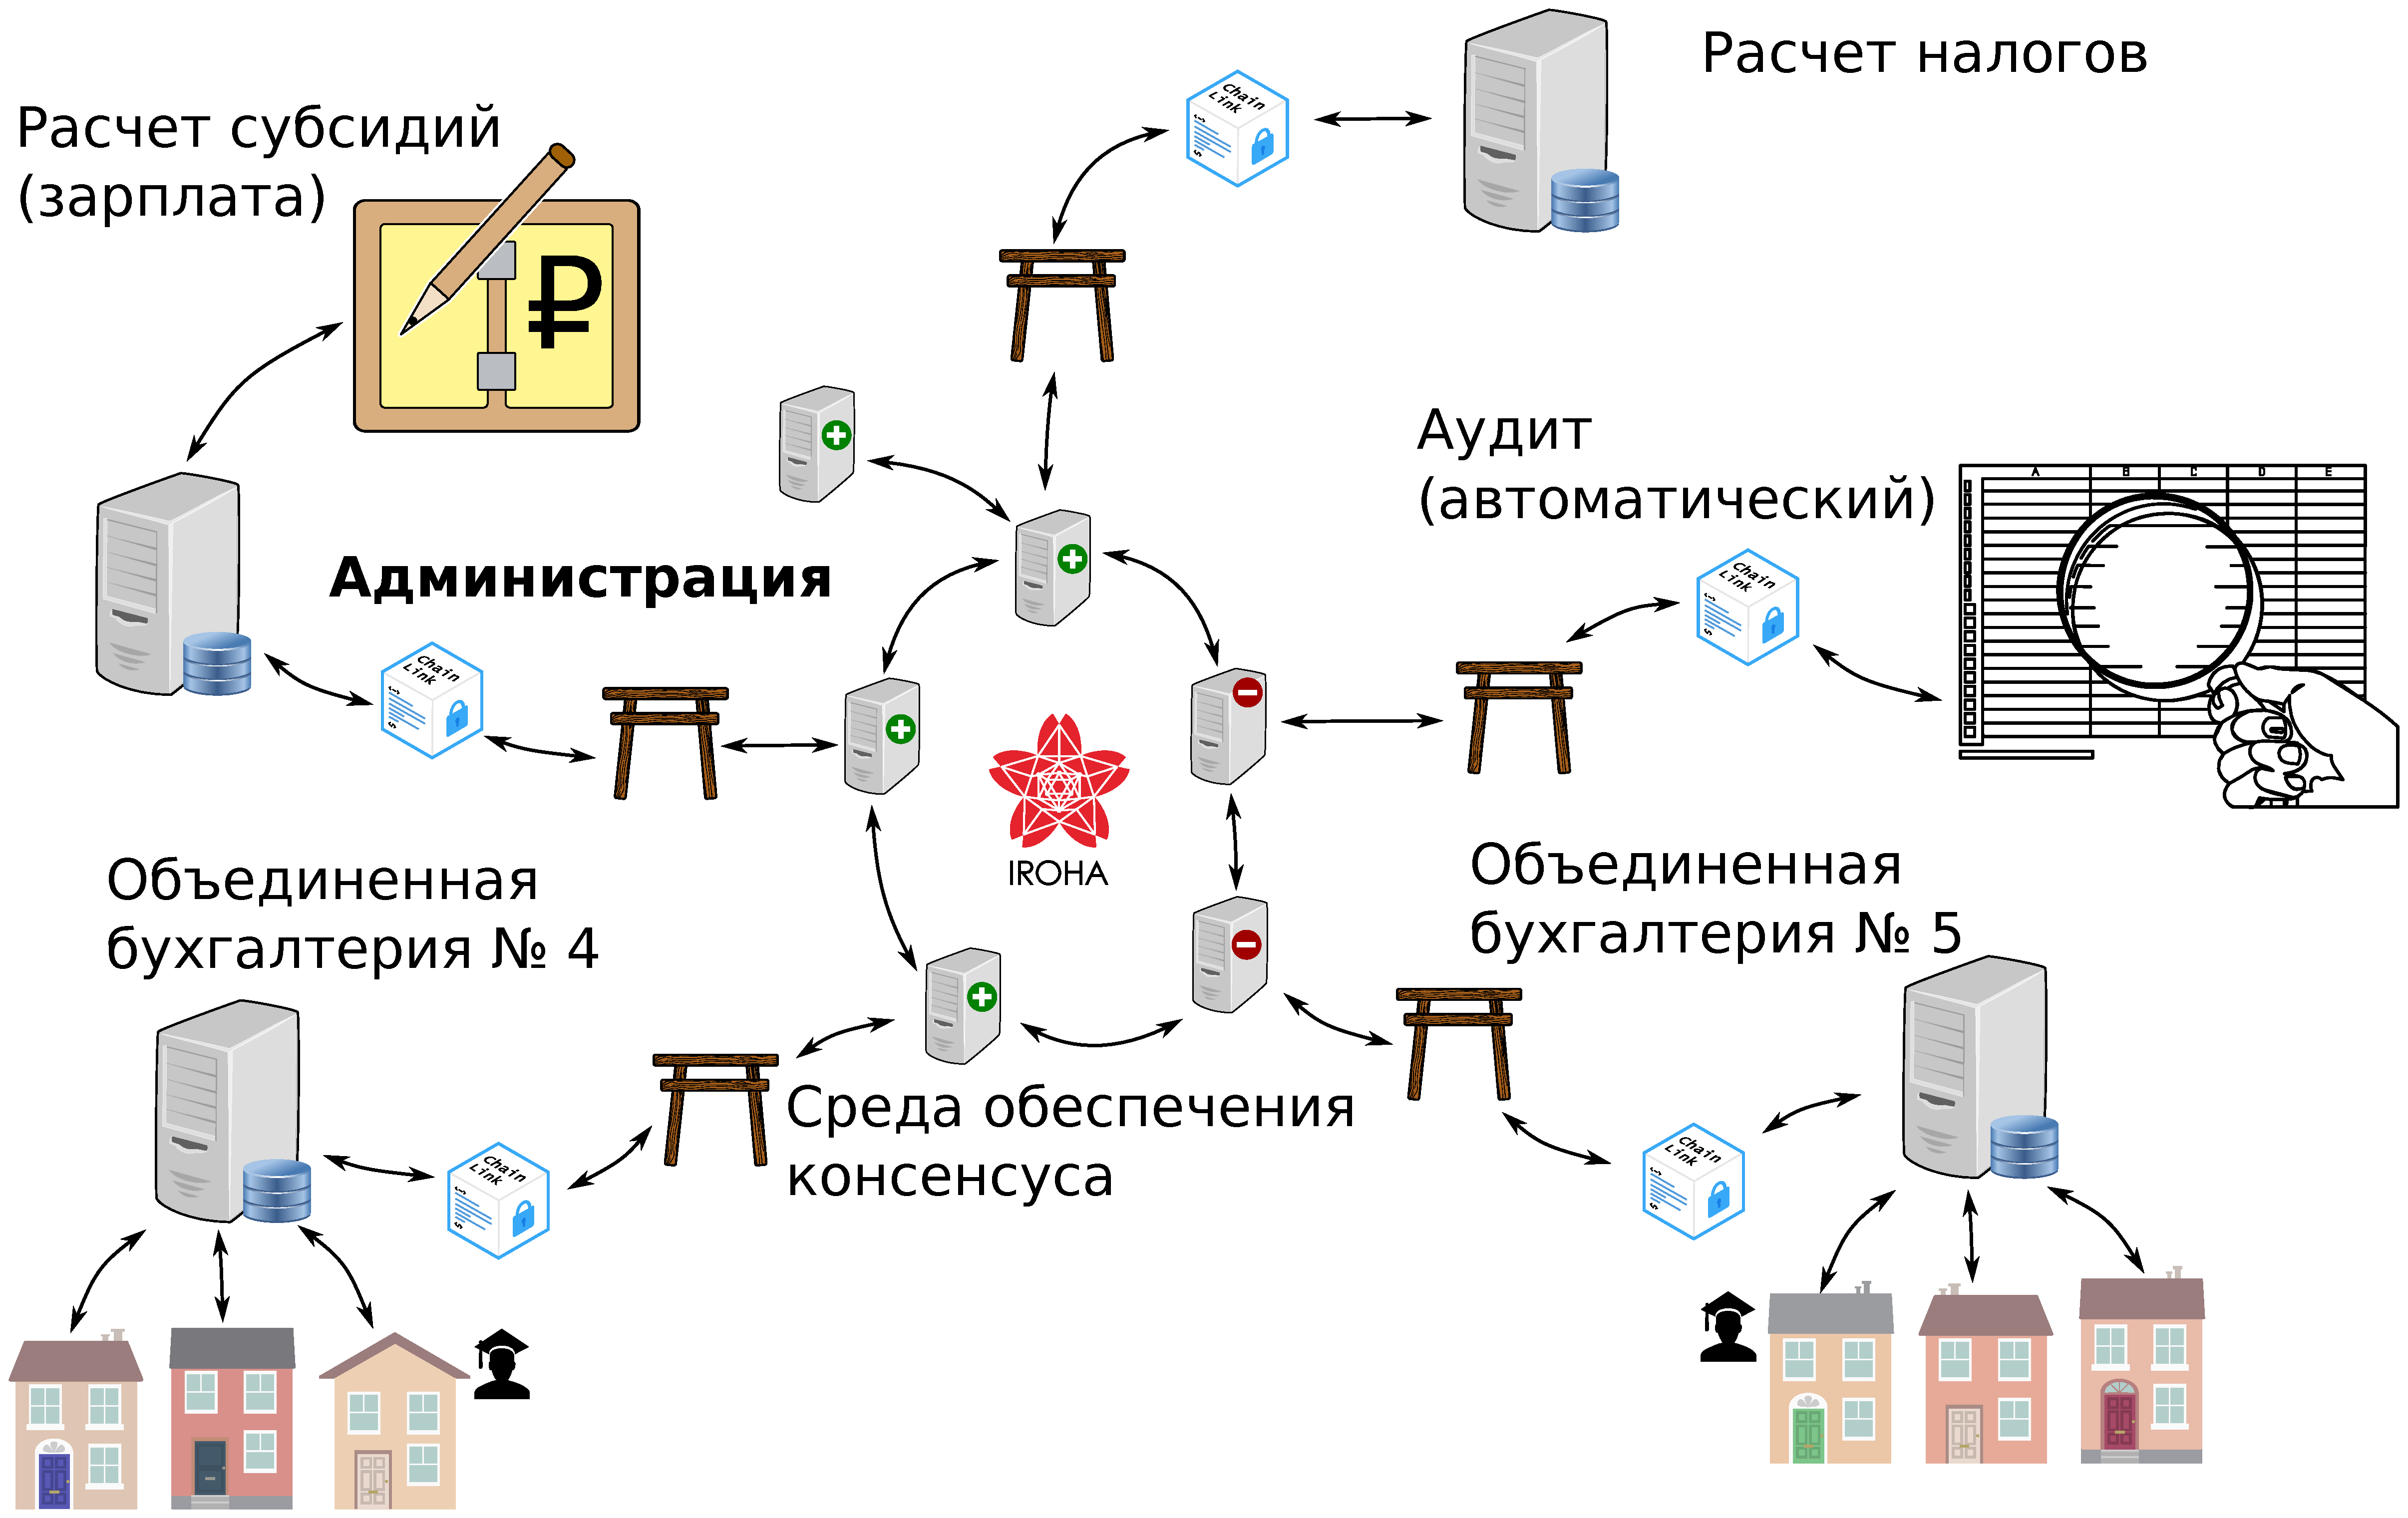
\includegraphics[width=1\linewidth]{pics/system-with-consensus.pdf}
\end{frame}

\begin{frame}[fragile]
  \frametitle{Интеграция данных}
  \begin{center}
      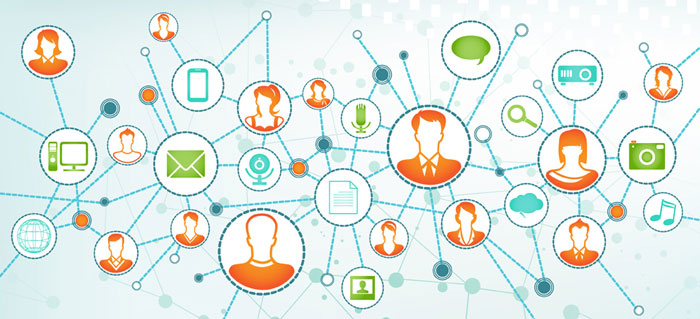
\includegraphics[width=0.5\linewidth]{pics/lod-pilot.jpg}
  \end{center}
  \begin{columns}
    \begin{column}{0.4\linewidth}
        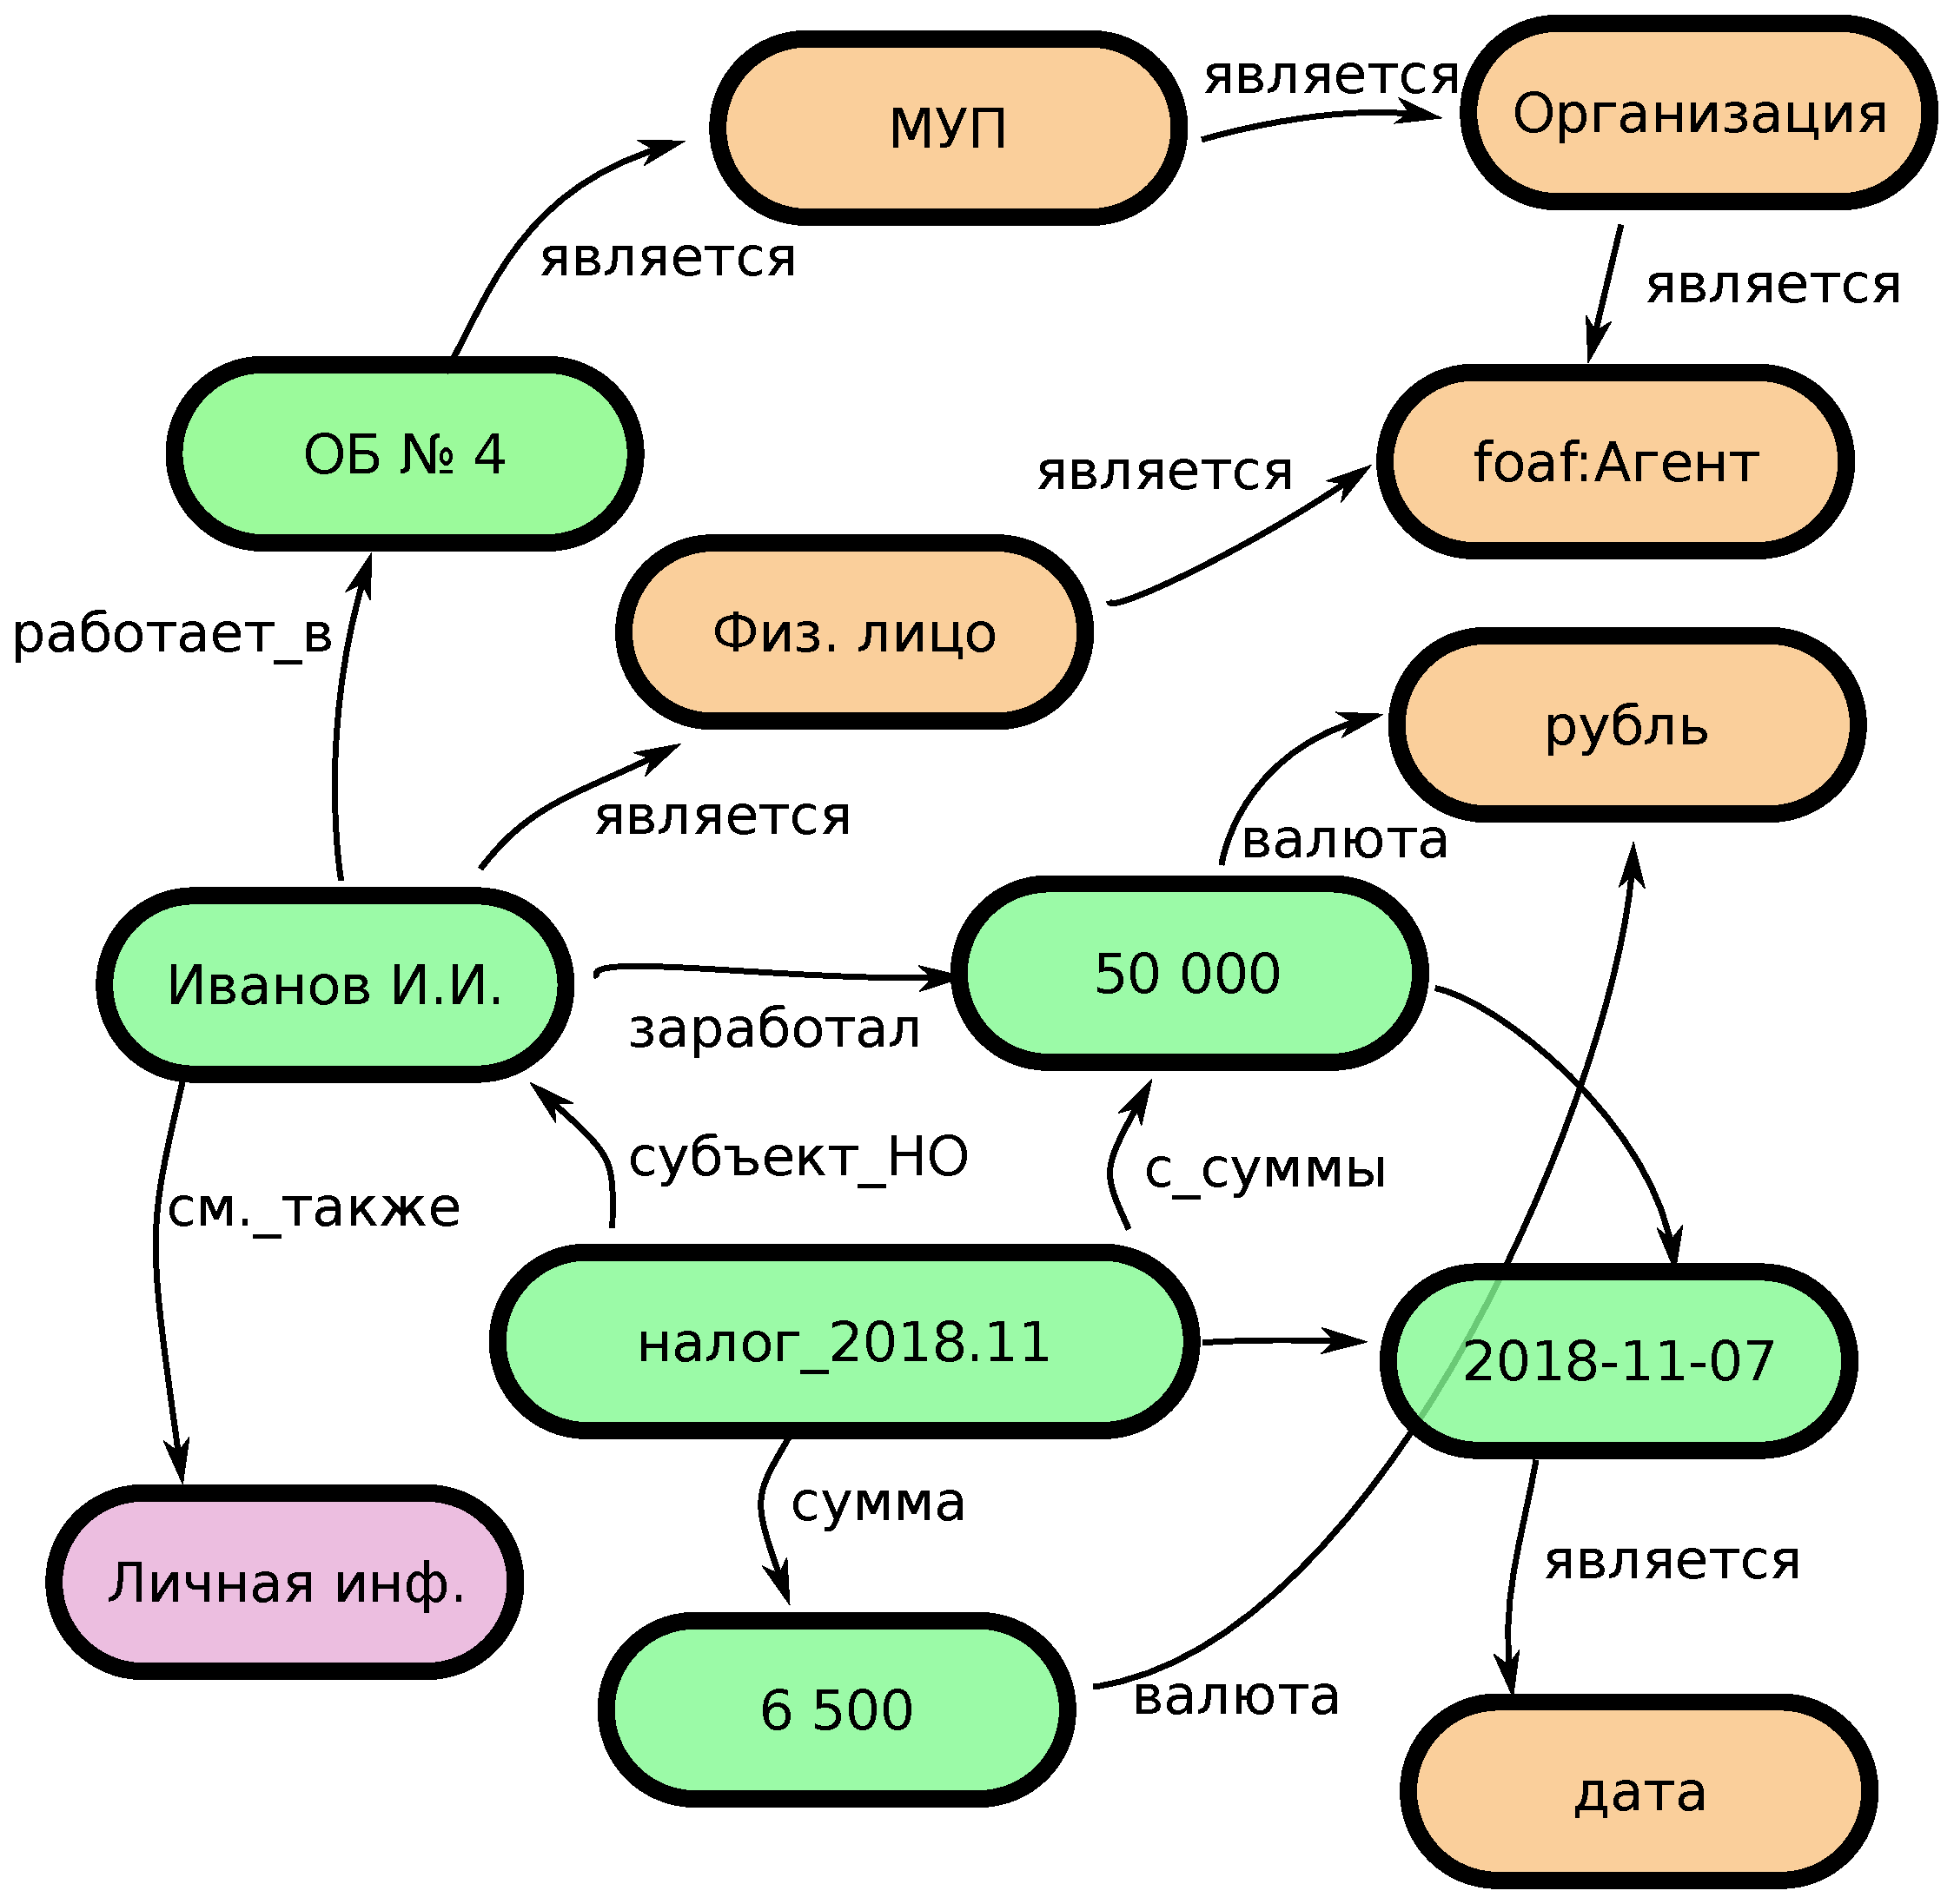
\includegraphics[width=1\linewidth]{pics/a-box.pdf}
    \end{column}
    \begin{column}{0.6\linewidth}
\begin{minted}{turtle}
@prefix dc: <http://purl.org/dc/elements/1.1/> .
@prefix rdf: <http://www.w3.org/1999/02/22-rdf-syntax-ns#> .
@prefix o: <http://www.admirk.ru/mup/accounting/4#>.

o:tax_2018.11 a eco:Taxation ;
    eco:hasSumm: o:summ_6000 ;
    eco:baseSumm: o:salary_50000 ;
    eco:taxSubject o:ivanov_i_i .

o:summ_50000 a eco:Rouble ;
    eco:summ: 50000 .

o:summ_6000 a eco:Rouble ;
    eco:summ: 6000 .

o:ivanov_i_i a foaf:Person ;
    dc:title "Иванов И.И." ;
    schema:worksIn o:muo_n_4 .
    rdfs:seeAlso: <https://ivanov.com/private_data#me>

o:muo_n_4 a foaf:Organization .
o:MUO a foaf:Organization .

foaf:Person a foaf:Agent .
foaf:Organization a foaf:Agent .

\end{minted}
    \end{column}
  \end{columns}
\end{frame}

\begin{frame}
  \frametitle{Производные технологии}
      На основе платформы можно разрабатывать:
      \begin{itemize}
      \item Системы автоматизации публикации размеченных данных;
      \item Автоматический документооборот с предприятиями (не внутренний, а глобальный);
      \item Сервисы расчета, анализа и аудита, агрегирования информации;
      \item Автоматизировать проектирование информационных систем:
        \begin{itemize}
        \item моделирование и синтез структуры базы данных;
        \item протоколы обмена данными с другими информационными системами;
        \item планировать вычислительные процедуры, и т.п.
        \end{itemize}
      \item \ldots
      \end{itemize}
\end{frame}

\begin{frame}
  \frametitle{Контактная информация}
  \begin{block}{}
    \begin{itemize}
    \item Черкашин Евгений Александрович, к.т.н., с.н.с. ИДСТУ СО РАН
    \item E-mail: \href{mailto:eugeneai@irnok.net}{\texttt{eugeneai@irnok.net}}
    \item Тел: +7 (914) 870-67-54
    \item \url{http://iscnet.ru:8080}
    \end{itemize}
  \end{block}
  % 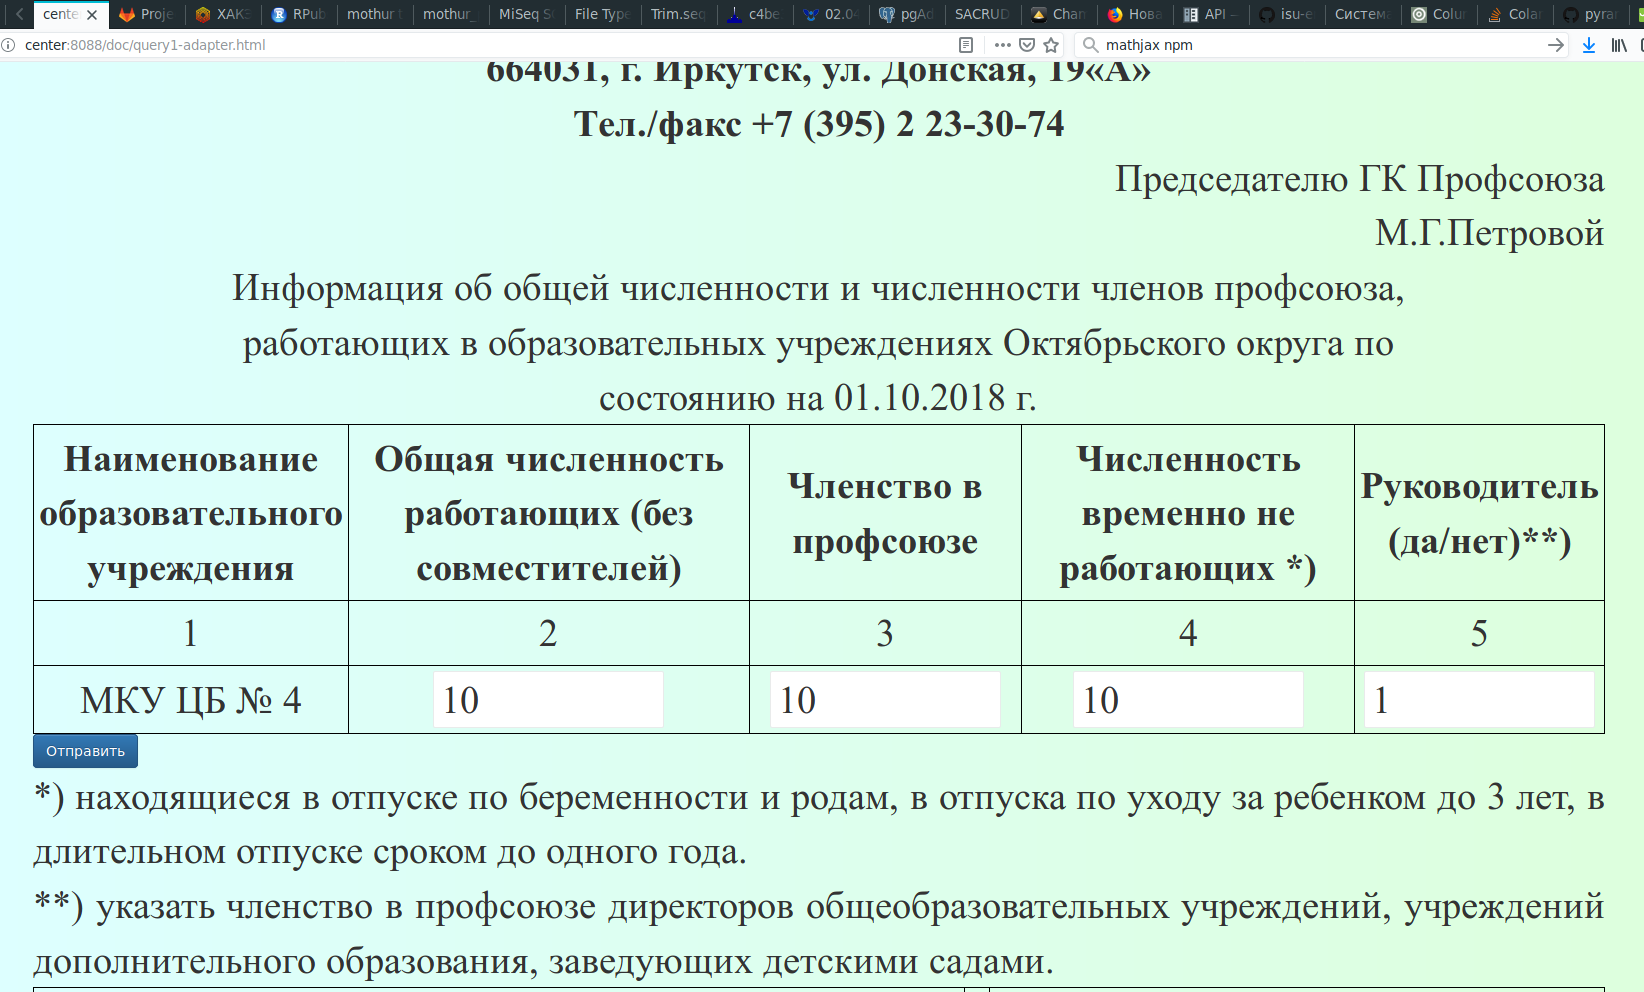
\includegraphics[width=1\linewidth]{pics/quest-form.png}
\end{frame}



% \begin{frame}
%   \vfill
%   \begin{center}
%     {\Huge Спасибо за внимание!}
%   \end{center}
%   \vfill
%   Исходный код (без документации) доступен на github.com: \url{https://github.com/isu-enterprise/icc.xmitransform}, \url{https://github.com/eugeneai/icc.mothurpim}.
% \end{frame}

\end{document}

%%% Local Variables:
%%% mode: latex
%%% TeX-master: t
%%% End:
